\documentclass{report}
\usepackage{lipsum} % for dummy text
\usepackage{draculatheme}
\usepackage{graphicx}
\usepackage{subfigure}
\usepackage{multirow}
\setcounter{secnumdepth}{0}

\title{Cubo - Memo}
\author{Botond Kovács, Frank Dierolf}

\begin{document}
\maketitle

\section{Introduction}

This document is a concise Buisness Plan.
It follows the 6 Page Memo Style, which got popular over Amazon's use in executive mettings.
I chose this structure because it inherits reading flow, aims executives and I feel comfortable with it.

First, let me introduce you to Cubo.
Cubo is a wooden cube, that you can place on every desk, coworking space, household and a great crafted piece of wood for every interior.
Cubo is also a Blockexplorer which adapts to the Users needs.
Cubo is the answer of Complexity and rooden language in the technology and especially the crypto space.
Cubo is a product of the Polkar - Team.
The team is combine of Botond, a Software Architect by profession and Frank, me, a Buisness Developer.

Before we outline the core elements, lets go back in time and tell our Backstory.

\section{The Backstory}
Franks story starts 3 years ago.
Crypto was just on the rise.
Me, Frank, just started out in conquering this area.
The first thing that stood appart compare to anything else that i encountered is, the language.
Its scary, unpleasant and feels wanna be smart in many corners.

Nontheless after a brief of time, i got used to it and adopted it.
The obvious happend. Another Problem appeared.
Noone understood me and to communicate crypto ideas to non crypto people is an nightmare.
Thats not the first time that i encounter this issue.
f.e. the medical industry shares the same issue.

I did, what i usually do. I simplify. Get rid of the ideas, get rid of the concepts, get rid of the buzzwords.
Get as close to the already known as possible. That leads to a point where i acquired a language thats catchy and understandable.
Even for Grandma.

It has a drawback. Its worth taking but a drawback nontheless.
Its not appealing for Business and Technology enviorment. People smile over this kind of communciation style.
But the right language lies where the market sits. The market sits in the everydays.
Things that people  buy in a supermarket, that people buy in a drug store, that people buy in amazon, that people buy ...

If Crypto wants high adoption, then lets switch gears and bring our great tools in every shelf, let people explore it by themselve and make money meanwhile.

Now, to the current time.
Botond and Me met on another Coding Competion. It was just us two in a team.
We had great fun together.
Admiration of each other was there from the get go.
Everyone throw something on the table, which the other person saw extrem rarely before.

We decided to go for another round, choose Dora Hacks Polkadot Hack and throw a coin for which category we are tackling.
Category Polkadot ecological developer tools.

\newpage

\section{Cubo}

We need an Idea. Botond came up with a AI blockexplorer.
You type what you want to get what you asked for.
I thought about an AR Cube. Holograms are sized, colored, animated based on Blockchain Data.
Inspired by one the sucess stories in the Auguemted Reality space, called Merge Cube.
So met in the middle and come up with Cubo.

Then we casted our spells, one after the other. We scratched Software Design Sheet.
We 3D Printed first Prototype.
We attach QR Codes.
We scratched ai driven visualtion engine, inspired templating engines.
We decided for going with search for configuration of visualtions.
We decided to add Dashboard Utilizies.
We redesign the Cube, lasered it out, stiched it togehter.
We scratch around in Figma for good intiutive layout and userfriendly UX.
We made simple user tests and collect some feedback.
We decided on a useful repo structure.
We added docs, presenation, buisnessplan, pitch deck to round it up.
2 weeks are gone, deadline is there and we are happy. Top notch timing for upcomming christmas.

\begin{figure}[hbp]
	\centering
	\subfigure[Configuarable Dashboard]{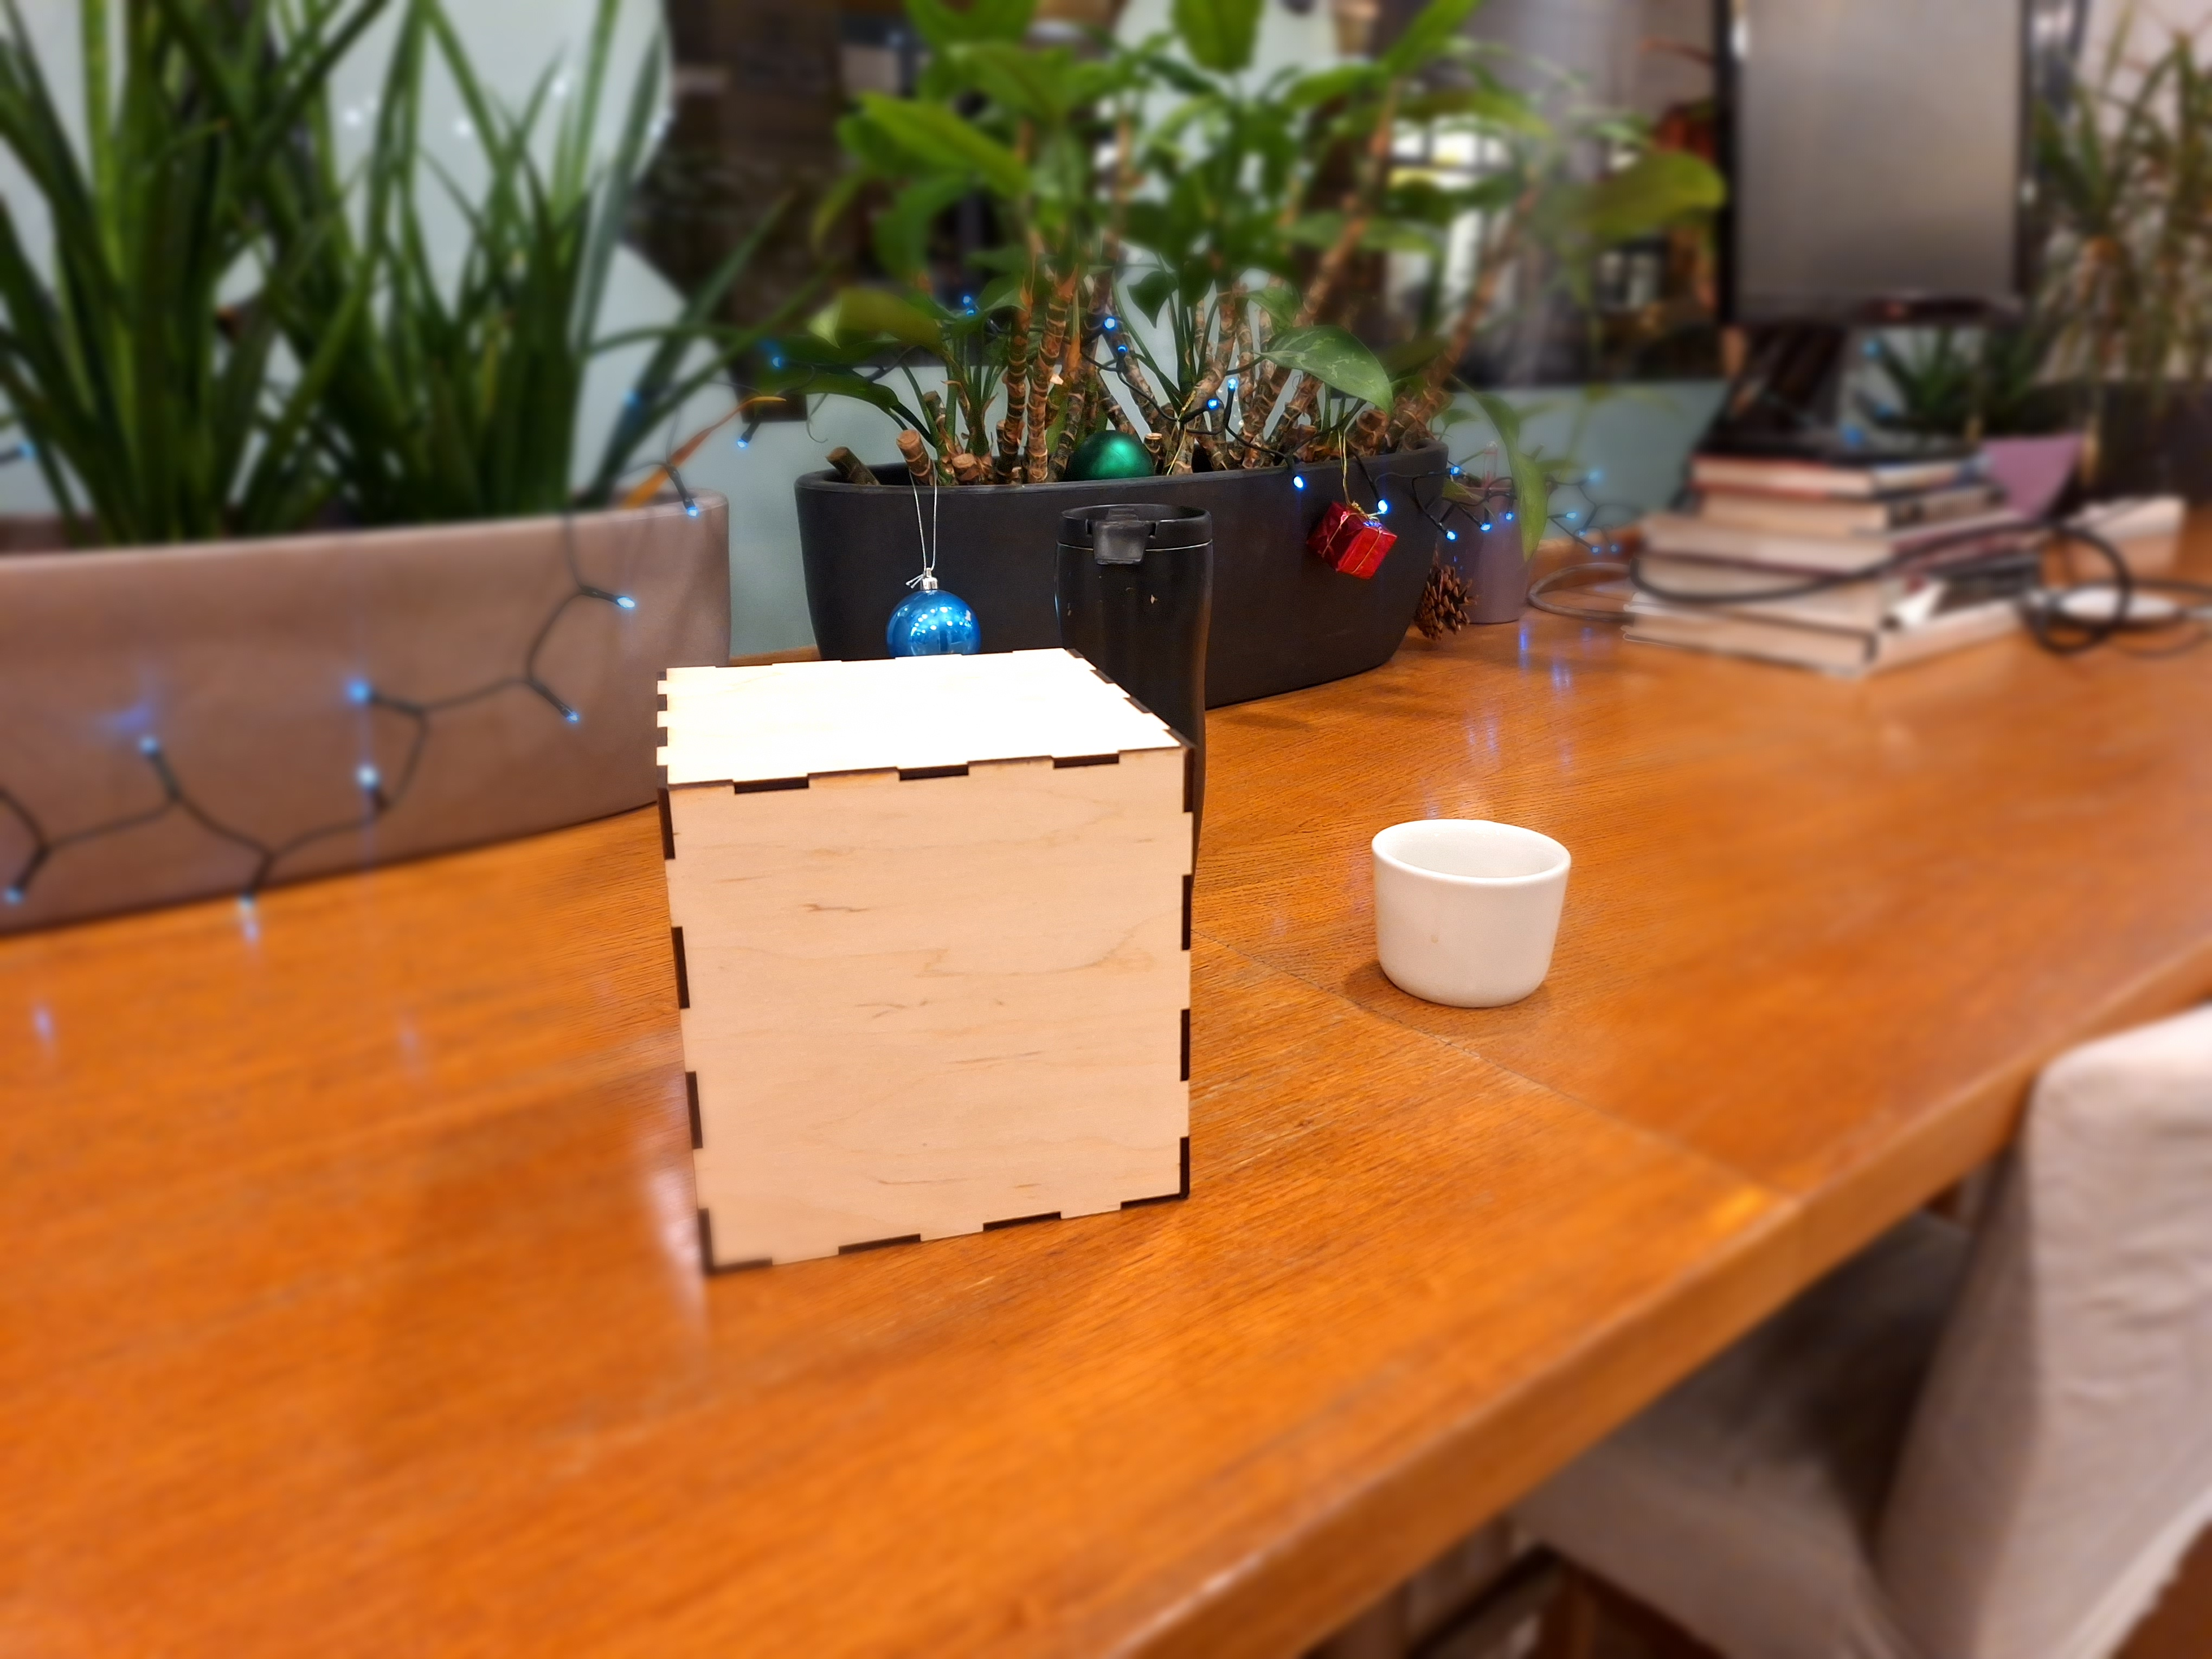
\includegraphics[width=0.4\textwidth]{./Cubo.jpg}}
	\hspace{1cm}
	\subfigure[Physical Product]{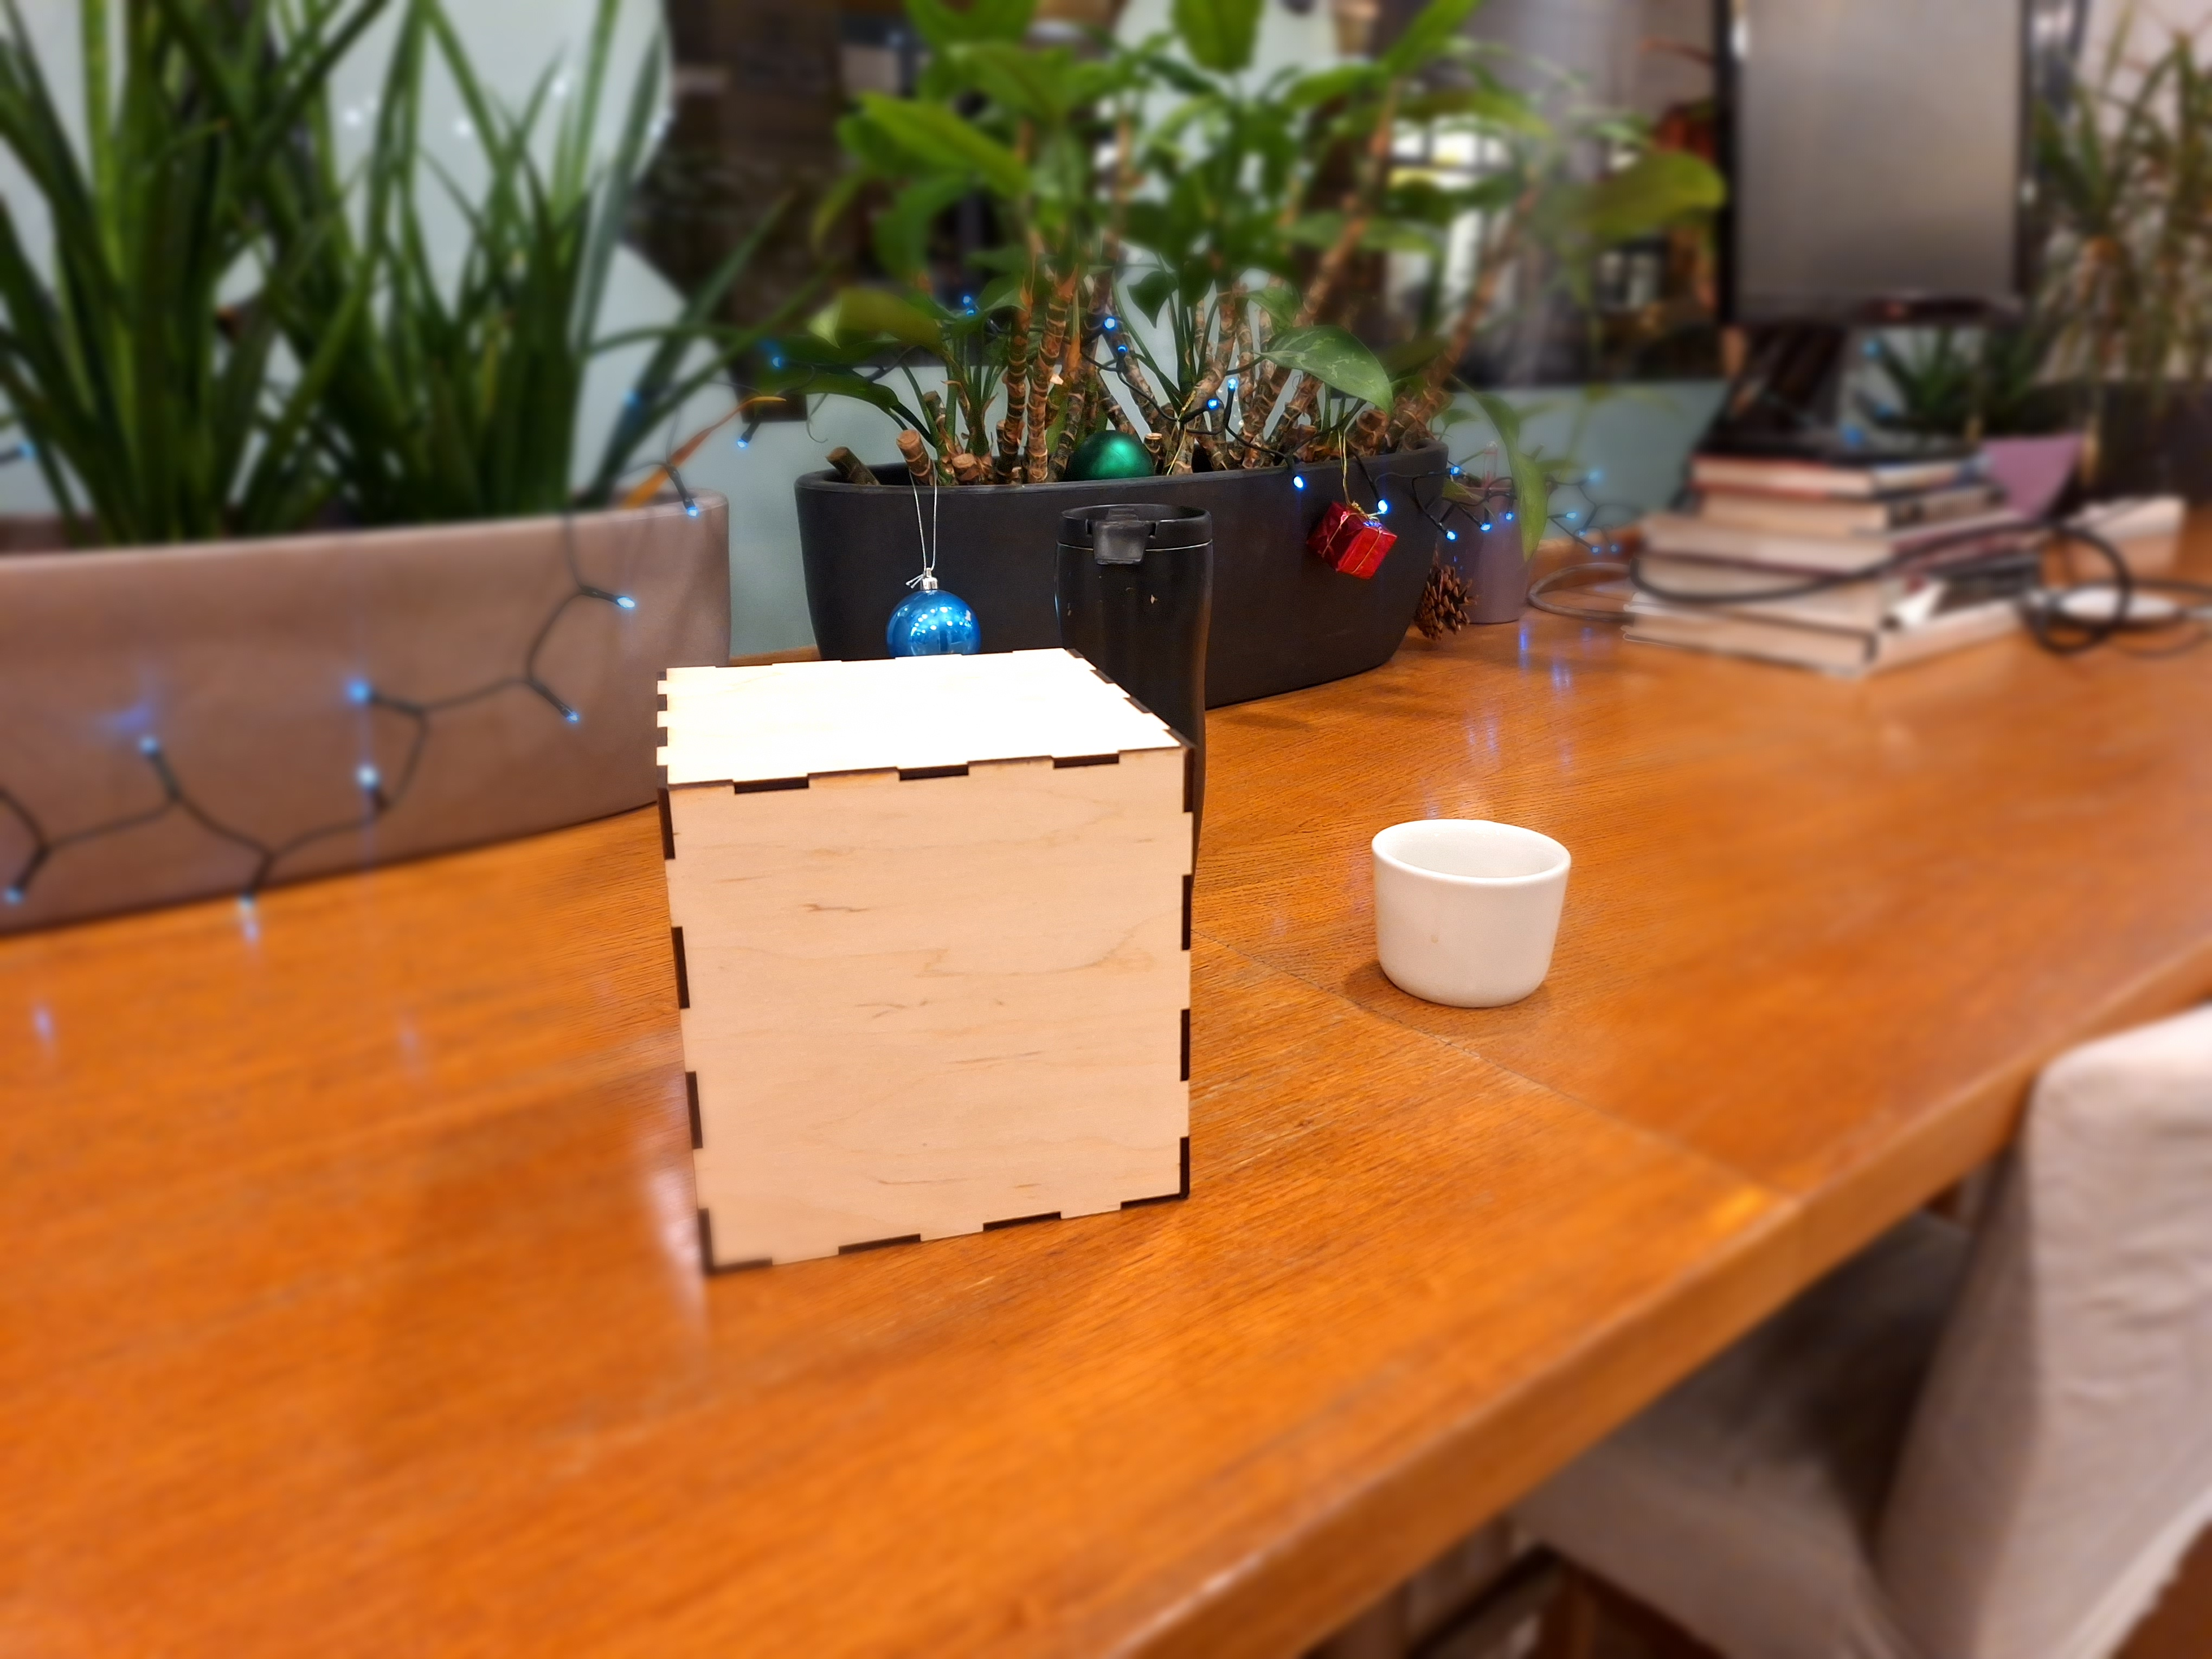
\includegraphics[width=0.4\textwidth]{./Cubo.jpg}}
	\caption{Cubo}
	\label{fig:Cubo}
\end{figure}

Back to buisness. How we plan to make money.
Like always, there are multiple tactics to approach a market.
I choose to structure the following section in Usersgroups.
Every Usergroup gets market approach.
Every buisness follows the following formula to reach sucess.
Earnings = Cost - income
So every market approach has a table which displays earnings, cost and income.

\newpage

\section{Tactics}

Usergroup A - Everyones: We sell Cubo's
\begin{table}[hbp]
	\centering
	\caption{Sales, Cost, and Earnings}
	\label{tab:sales}
	\begin{tabular}{|c|c|c|}
		\hline
		\textbf{Sold} & \textbf{Cost} & \textbf{Earning} \\
		\hline
		1             & \$10          & \$40             \\
		\hline
		10            & \$100         & \$400            \\
		\hline
		100           & \$1000        & \$4000           \\
		\hline
		1000          & \$10000       & \$40000          \\
		\hline
		10000         & \$100000      & \$400000         \\
		\hline
	\end{tabular}
\end{table}
\\
Selling Cubos is the simplest approach.
It aims for the everyones.
Cubo gets seen as a nice piece of Furniture with Holograms.
Cubo seen as Blockexplorer is not important.

The Market approach is take the phone, call people and extend on it.
It does the thing.
Calling friends on the first day and ask if they wanna buys a cubo.
That leads the following: In the first day 10 leads, in a week 70 leads, in a month I have 240.
Scaling via social media and creating content to build a base.
Further scaling via offering other plattforms, ebay, etsy, amazon.
Always collecting feedback and input.

Iterate and listen is underlying philosphy.

\vspace{2em}

\hspace{-1em}Group B - Techies: We sell Access Tokens
\begin{table}[hbp]
	\centering
	\caption{Sales, Cost, and Earnings}
	\label{tab:sales}
	\begin{tabular}{|c|c|c|}
		\hline
		\textbf{Sold} & \textbf{Cost} & \textbf{Earning} \\
		\hline
		1             & \$1           & \$1              \\
		\hline
		10            & \$2           & \$10             \\
		\hline
		100           & \$3           & \$100            \\
		\hline
		1000          & \$4           & \$1000           \\
		\hline
		10000         & \$5           & \$10000          \\
		\hline
	\end{tabular}
\end{table}
\\
\lipsum[1][1-10]

\newpage

\section{Market Strategy and Timeline}
\section{Conclusion}
\end{document}
